\documentclass[tikz,border=8pt]{standalone}
% Shared styles for the Hands-On 4 diagrams. Colours match the Hands-On 1 diagrams.
\usepackage{amsmath,amssymb}
\usetikzlibrary{positioning,calc,arrows.meta,decorations.pathreplacing,shapes.geometric}
\definecolor{tensorblue}{HTML}{3274B5}
\definecolor{envblue}{HTML}{1E4C7C}
\definecolor{opteal}{HTML}{357A76}
\tikzset{
  leg/.style={line width=1.7pt},
  thinedge/.style={line width=1.0pt},
  tensor/.style={circle,draw,line width=1.5pt,fill=tensorblue,minimum size=9mm,inner sep=0},
  vertex/.style={circle,draw,line width=1.0pt,fill=white,minimum size=6mm,inner sep=0,font=\small},
  copy/.style={circle,draw,line width=1.5pt,fill=black,minimum size=3.6mm,inner sep=0},
  op/.style={rectangle,draw,line width=1.5pt,fill=opteal,minimum size=5.6mm,inner sep=0},
  % messages are triangles pointing in the direction the message travels
  msg/.style={isosceles triangle,isosceles triangle apex angle=75,draw,line width=1.5pt,fill=envblue,inner sep=0,
              minimum width=8mm,minimum height=10mm,shape border rotate=0},
  msgl/.style={msg,shape border rotate=180},
  msgu/.style={msg,shape border rotate=90},
  msgd/.style={msg,shape border rotate=270},
  % a matrix message: a slightly larger triangle, its two legs fan out from it
  msgmat/.style={msg,minimum width=10mm,minimum height=13mm},
  lab/.style={font=\large},
  code/.style={font=\ttfamily\large},
  arrow/.style={-{Latex[length=3mm]},line width=1.2pt},
}

\begin{document}
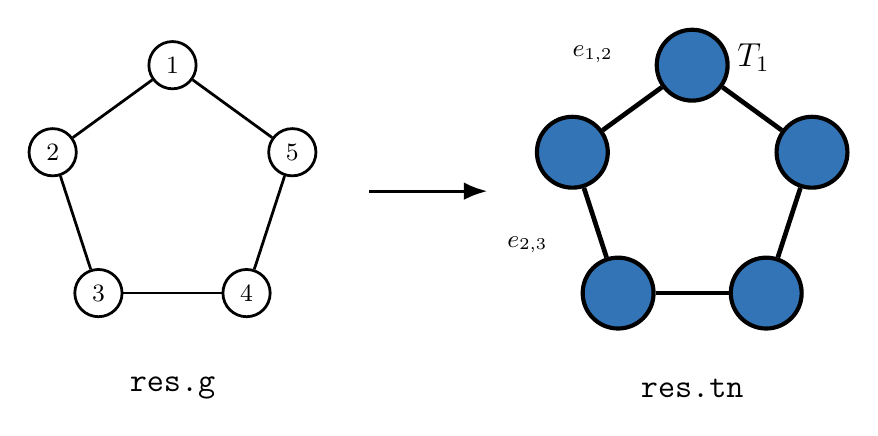
\begin{tikzpicture}
  % the graph g: a periodic path on 5 vertices
  \begin{scope}
    \foreach \i in {1,...,5} {
      \node[vertex] (g\i) at ({90+72*(\i-1)}:1.6) {$\i$};
    }
    \foreach \i/\j in {1/2,2/3,3/4,4/5,5/1} { \draw[thinedge] (g\i) -- (g\j); }
    \node[code] at (0,-2.5) {res.g};
  \end{scope}
  \draw[arrow] (2.5,0) -- (4.0,0);
  % the tensor network: one tensor per vertex, one shared index per edge
  \begin{scope}[xshift=6.6cm]
    \foreach \i in {1,...,5} {
      \node[tensor] (t\i) at ({90+72*(\i-1)}:1.6) {};
    }
    \foreach \i/\j in {1/2,2/3,3/4,4/5,5/1} { \draw[leg] (t\i) -- (t\j); }
    \node[lab] at ({90+36}:2.15) {\small$e_{1,2}$};
    \node[lab] at ({90+72+36}:2.2) {\small$e_{2,3}$};
    \node[lab,anchor=west] at ($(t1)+(0.45,0.1)$) {$T_1$};
    \node[code] at (0,-2.5) {res.tn};
  \end{scope}
\end{tikzpicture}
\end{document}
